\documentclass[11pt,letterpaper]{article}
\usepackage[margin=0.9in,headheight=14pt,headsep=18pt]{geometry}
\usepackage{iftex}
\ifPDFTeX
  \usepackage[T1]{fontenc}
  \usepackage[utf8]{inputenc}
  \usepackage{lmodern}
\else
  \usepackage{fontspec}
  \setmainfont{lmroman10-regular.otf}[BoldFont=lmroman10-bold.otf,
    ItalicFont=lmroman10-italic.otf,BoldItalicFont=lmroman10-bolditalic.otf]
  \setmonofont{lmmono10-regular.otf}[Scale=0.88]
\fi
\usepackage{microtype}
\usepackage{amsmath,amssymb}
\usepackage{graphicx}
\usepackage{longtable,booktabs,array,calc}
% Pandoc 3.11 uses LTcaptype=none for uncaptioned tables. Older TeX bundles
% still advance that counter; define it without affecting numbered captions.
\newcounter{none}
\usepackage{etoolbox}
\usepackage{caption}
\usepackage{fancyhdr}
\usepackage{titlesec}
\usepackage{xcolor}
\definecolor{linkink}{HTML}{245B78}
\usepackage{xurl}
\usepackage[colorlinks=true,allcolors=linkink,breaklinks=true]{hyperref}
\hypersetup{pdftitle={What Does a Glucose Foundation Model Understand
About Me?},pdfauthor={Ibraim Abduramanov},pdfsubject={A Single-Person
Test of Frozen OpenCGM-StateEvent Embeddings}}
\urlstyle{same}
\setlength{\emergencystretch}{2em}
\setlength{\parindent}{0pt}
\setlength{\parskip}{0.2em}
\setlength{\LTpre}{0.4em}
\setlength{\LTpost}{0.7em}
\AtBeginEnvironment{longtable}{\small\renewcommand{\arraystretch}{1.12}}
\captionsetup{font=small,labelfont=bf,justification=justified,singlelinecheck=false}
\titleformat{\section}{\large\bfseries}{}{0pt}{}
\titleformat{\subsection}{\normalsize\bfseries}{}{0pt}{}
\titlespacing*{\section}{0pt}{1.2em}{0.45em}
\titlespacing*{\subsection}{0pt}{0.9em}{0.3em}
\setcounter{secnumdepth}{-1}
\providecommand{\tightlist}{\setlength{\itemsep}{0pt}\setlength{\parskip}{0pt}}
\providecommand{\pandocbounded}[1]{#1}
\pagestyle{fancy}
\fancyhf{}
\fancyhead[L]{\footnotesize Frozen OpenCGM embeddings for personal glucose forecasting}
\fancyhead[R]{\footnotesize Working preprint}
\fancyfoot[C]{\small\thepage}
\renewcommand{\headrulewidth}{0.3pt}
\begin{document}
\thispagestyle{plain}
\begin{center}
{\LARGE\bfseries What Does a Glucose Foundation Model Understand About
Me?\par}
\vspace{0.65em}
{\large A Single-Person Test of Frozen OpenCGM-StateEvent
Embeddings\par}
\vspace{1em}
{\normalsize Ibraim Abduramanov\par}
\vspace{0.35em}
{\small Working preprint --- 21 September 2026\par}
\end{center}
\vspace{0.45em}
\begin{abstract}
\noindent A frozen glucose encoder did not establish added forecasting
value beyond eight glucose/time summaries in this retrospective
self-study. The experiment evaluates one public OpenCGM-StateEvent
checkpoint, an independent community reconstruction of the GlucoFM
method, on the author's continuous glucose monitoring history. Fifteen
CareLink exports contain 338,084 distinct local glucose timestamps
across May 2023--September 2026. An audit identified 24 conflicting
timestamps on two clock-change days; a conservative rule excluded
windows touching any recorded clock-change day. The resulting 11,044
eligible windows support a temporally separated comparison of
persistence, glucose-summary Ridge, and the same Ridge predictor
augmented with 128 frozen encoder features. Preprocessing, splits,
tuning and the primary outcome were recorded before scores were
inspected. On 654 later-test windows across 12 weeks, 60-minute mean
absolute error was 42.59 mg/dL for persistence, 37.66 for summary Ridge
and 37.36 for augmented Ridge. The paired augmented-minus-summary
difference was \ensuremath{-}0.30 mg/dL (95\% week-bootstrap interval \ensuremath{-}0.87 to
+0.34). All eight horizon-by-period intervals included zero; several
point estimates favored the simpler model. The result is limited to one
individual, one community checkpoint and one forecasting protocol; it is
neither an evaluation of Google's weights nor evidence of equivalence or
physiological understanding.
\end{abstract}
\vspace{0.4em}
\section{1. Introduction}\label{introduction}

At the primary 60-minute horizon, a frozen 128-dimensional glucose
embedding reduced error by only 0.30 mg/dL beyond eight glucose and
time-of-day summaries, with uncertainty spanning both improvement and
deterioration. That narrow result answers the practical question behind
this study: did the representation earn its place in a predictor of this
person's glucose?

The author reports living with type 1 diabetes for 17 years and managing
his own closed-loop therapy. GlucoFM {[}1{]} provided the motivation to
ask whether a model learned from other people's glucose recordings could
add useful information about his own history. The paper reports a
dual-stream representation of slower glucose state and faster events,
followed by frozen-feature downstream evaluations. Its reported results
are not reproduced here.

A bounded source search did not locate a verified official Google
checkpoint. The present experiment therefore uses the explicitly
identified OpenCGM-StateEvent community release {[}2, 3{]}. Its model
card describes an independent reconstruction trained on public cohorts.
It is a distinct empirical object: evaluating it does not test Google's
checkpoint or establish whether the original paper's results reproduce.

The operational question is deliberately smaller than the title:
\textbf{do frozen encoder features improve a linear predictor that
already receives summaries of the same observed glucose history?} All
arms share issue times, history, outcomes and temporal splits. The
comparison tests incremental forecasting utility within a fixed model
family. It does not test the causal meaning of the representation or the
author's response to model advice.

The contribution is a measured negative result with an auditable chain
from export semantics to paired forecast errors. Two details matter to
that chain: conflicting wall-clock timestamps cannot be resolved by
silently keeping the first row, and midnight insulin aggregates cannot
stand in for timestamped deliveries. These observations determined the
eligible data before any encoder comparison score was examined.

\textbf{Evidence convention.} Numerical findings in this manuscript are
measured outputs of the commands in Appendix B. Claims about the
original model and community pretraining are attributed to their
sources. Missing ordering evidence and limits of inference are stated
explicitly. The evaluation specification was frozen locally in
\texttt{TANDEM.md} before scoring; it was not an externally registered
protocol.

\section{2. Personal archive and measurement
boundaries}\label{personal-archive-and-measurement-boundaries}

\subsection{2.1. Archive coverage and clock
ambiguity}\label{archive-coverage-and-clock-ambiguity}

Fifteen non-overlapping CareLink CSV exports contain 402,385 dated event
rows and 338,084 distinct local glucose timestamps from 9 May 2023 to 20
September 2026. Glucose readings occur on 1,227 days. The inventory
distinguishes coverage inspection from forecasting: inspecting an export
does not make a later score an untouched prospective result.

There are 24 timestamps with conflicting glucose values on two days
containing recorded pump-clock changes. Across the archive, 17
clock-change rows populate only \texttt{Index}, \texttt{Date},
\texttt{Time} and \texttt{New\ Device\ Time}. None of the conflicting
glucose pairs brackets a clock-change row by export index. Neither those
fields nor export order establish a verified monotone acquisition
timeline or UTC offset.

The implemented rule rejects any window whose full support, from 24
hours before issue to 122.5 minutes after issue, touches a conflict day
or any calendar day between a clock-change row's old and new dates,
inclusive. This excludes 17 calendar days and 399 candidate windows. It
is intentionally broader than deleting the 24 colliding timestamps:
histories crossing a clock adjustment can have uncertain elapsed-time
meaning even when their timestamps are unique. Original records are
preserved. All 15 CSV hashes still match the pre-experiment inventory.

\subsection{2.2. Insulin semantics and
scope}\label{insulin-semantics-and-scope}

All 1,200 {\ttfamily\nolinkurl{CLOSED_LOOP_AUTO_INSULIN}} rows in these exports
occur at midnight. They are treated as daily aggregates, not timestamped
insulin deliveries. The present comparison uses only glucose and local
time of day; neither those aggregates nor carbohydrate or bolus records
enter its predictors.

An earlier project experiment evaluated recorded carbohydrates and prior
boluses at meal-related issue times. It used a different archive,
population and tuning design. Its results and corrected feature errors
remain in the historical record, but its scores are not pooled with this
comparison. The current fixed-time sampling also avoids excluding a
forecast because another meal will occur after it. Requiring complete
future glucose observation still introduces selection, as discussed in
Section 5.

\section{3. Evaluation design}\label{evaluation-design}

\subsection{3.1. History, outcomes and
eligibility}\label{history-outcomes-and-eligibility}

Forecasts are issued every two hours on the pump-local wall clock. Let
\(t\) be an issue time and \(s=t-24\,\mathrm{h}\) its history start.
Each model receives the same oldest-first 288-position history. Observed
glucose is converted from mmol/L to mg/dL using the existing conversion
factor 18.0182. Source timestamps in \([s,t)\) are assigned to positions
by

\[
j=\left\lfloor\frac{\tau-s}{5\,\mathrm{min}}+\frac{1}{2}\right\rfloor,
\qquad j\in\{0,\ldots,287\}.
\]

Readings assigned to the same position are averaged; indices outside
this range are discarded. This follows the pinned source implementation
{[}3{]}. Missing positions have value zero and mask zero. Observed
positions have mask one. There is no interpolation or external
per-window normalization. The clock exclusions are applied before
binning, so conflicting raw timestamps are never averaged into a model
input.

Eligibility requires at least 80\% observed bins over the full history
and its final three hours, an observed final bin, and no raw history gap
longer than 60 minutes, including the history edges. The minimum
full-history count among retained windows was 270 of 288 observed bins;
the other rules can be stricter than the nominal coverage threshold.

Targets are means of observed readings in half-open bins
\([t+h-2.5\,\mathrm{min},t+h+2.5\,\mathrm{min})\). All 24 five-minute
future bins must be observed. The evaluated horizons are 30, 60, 90 and
120 minutes, with identical samples at every horizon. Targets therefore
have a stated temporal tolerance; they are not asserted to be exact-time
measurements. The last history bin is centered five minutes before
issue, so persistence also uses that bin rather than a new reading at
issue time.

\textbf{Table 1. Measured eligibility flow.} Exclusions are sequential
and mutually exclusive in the listed order.

{\def\LTcaptype{none} % do not increment counter
\begin{longtable}[]{@{}lrr@{}}
\toprule\noalign{}
Stage & Removed & Remaining \\
\midrule\noalign{}
\endhead
\bottomrule\noalign{}
\endlastfoot
Fixed two-hour candidate issue times & --- & 14,754 \\
Incomplete archive-boundary support & 14 & 14,740 \\
Clock-ambiguity support overlap & 399 & 14,341 \\
History gap longer than 60 minutes & 2,939 & 11,402 \\
History coverage or final-bin failure & 103 & 11,299 \\
Missing future target bins & 255 & 11,044 \\
\end{longtable}
}

\subsection{3.2. Checkpoint identity and feature
extraction}\label{checkpoint-identity-and-feature-extraction}

The evaluated artifact is {\ttfamily\nolinkurl{sfourdrinier/opencgm-stateevent}},
Hugging Face revision {\ttfamily\nolinkurl{6c53e572c2dafcb0b030f2e1aa4f3a2a8d7f7ca3}}.
Its ONNX encoder is byte-identical to the encoder stored at GitHub
source revision {\ttfamily\nolinkurl{bcf8ac2dfca00f8fb3c7728fb2a3a2bd2803bebf}}.
Appendix A records the full encoder digest and runtime contract.

The maintainer identifies this artifact as seed 17, epoch 40, trained
with raw glucose statistics and {\ttfamily\nolinkurl{zero_empty_patches=false}}
{[}2{]}. The card's separate five-seed, 120-epoch evaluation is not
evidence about the exact file used here. Its public-cohort pretraining
description remains maintainer-reported; this study verifies file
identity and local behavior, not the training history.

Inputs are float32 glucose and mask arrays of shape \(B\times288\), plus
an int64 local circadian start index of shape \(B\). The released graph
performs observed-only instance normalization, state/event processing
and contextual encoding. Raw-mg/dL patch statistics also enter the
encoder, so externally standardizing glucose would change its documented
contract. The returned \(B\times128\) embedding is the unweighted mean
of 24 contextual tokens from the frozen online branch. We use the
released ONNX graph directly; rebuilding with current source defaults
would change its empty-patch behavior.

Synthetic graph and inference checks preceded private inference.
Constant, ramp, sparse, empty and partially masked histories produced
finite embeddings. Repeated calls were deterministic; batch-size and
finite masked-fill checks agreed. All private inference then ran locally
through the CPU provider. No encoder parameter or bundled probe head was
fitted to the author's records.

\subsection{3.3. Matched predictors and temporal
fitting}\label{matched-predictors-and-temporal-fitting}

\textbf{Persistence} predicts the final observed history-bin value at
every horizon. \textbf{Summary Ridge} uses eight features: that value;
observed-history mean, sample standard deviation, minimum and maximum; a
least-squares slope over the last six bins in mg/dL per minute; and
sine/cosine of issue time. \textbf{Augmented Ridge} uses those same
eight features plus all 128 frozen embedding dimensions.

Each Ridge model minimizes

\[
\sum_{i\in\mathcal{T}}(y_{i,h}-b_h-z_i^\top\beta_h)^2
+\alpha_h\lVert\beta_h\rVert_2^2,
\]

where \(z_i\) contains columns standardized with training-set means and
population standard deviations. The intercept is unpenalized. There is
no PCA, target normalization or prediction clipping. Each arm and
horizon selects its own regularization value from the same 19 log-spaced
candidates, \(10^{-3}\) through \(10^6\), by minimum event-weighted
validation MAE; ties select the smaller value.

\textbf{Table 2. Measured temporal populations.} Every boundary
condition applies to complete history or target support, not merely the
issue date.

{\def\LTcaptype{none} % do not increment counter
\begin{longtable}[]{@{}
  >{\raggedright\arraybackslash}p{(\linewidth - 4\tabcolsep) * \real{0.3000}}
  >{\raggedright\arraybackslash}p{(\linewidth - 4\tabcolsep) * \real{0.3000}}
  >{\raggedleft\arraybackslash}p{(\linewidth - 4\tabcolsep) * \real{0.4000}}@{}}
\toprule\noalign{}
\begin{minipage}[b]{\linewidth}\raggedright
Population
\end{minipage} & \begin{minipage}[b]{\linewidth}\raggedright
Support condition
\end{minipage} & \begin{minipage}[b]{\linewidth}\raggedleft
Windows
\end{minipage} \\
\midrule\noalign{}
\endhead
\bottomrule\noalign{}
\endlastfoot
Development training & Target support ends before 1 Jan 2025 & 5,334 \\
Validation & History starts on/after 1 Jan 2025; target support ends
before 1 Jan 2026 & 3,357 \\
Final training & All target support ends before 1 Jan 2026 & 8,704 \\
Exploratory test & History starts on/after 1 Jan 2026; target support
ends before 1 Jul 2026 & 1,662 \\
Later retrospective test & History starts on/after 1 Jul 2026; targets
available in the archive & 654 \\
\end{longtable}
}

After tuning, scaling and Ridge coefficients are refitted on final
training only and frozen for both test periods. Thirteen windows purged
between development training and validation rejoin final training; 24
eligible windows at test boundaries remain unused. Complete-support
purging prevents shared readings across the fitted-training/test
boundary. Overlap within each temporal population remains.

Earlier forecasting work examined March--June 2026, so the whole
January--June test is labeled exploratory. July--September had coverage
and export inspection but no recorded prior forecast comparison. It is a
later retrospective test, not a pristine prospective holdout. The
specification was recorded before comparison scores were inspected, and
no score-driven change to the protocol followed.

\subsection{3.4. Primary estimand and
uncertainty}\label{primary-estimand-and-uncertainty}

The primary outcome is the later-test difference in 60-minute MAE
between augmented and summary Ridge:

\[
\Delta_{60}=\frac{1}{n}\sum_{i=1}^{n}
\left(\lvert\hat y^{\mathrm{aug}}_{i,60}-y_{i,60}\rvert
-\lvert\hat y^{\mathrm{sum}}_{i,60}-y_{i,60}\rvert\right).
\]

Negative values favor embeddings. Each test slice uses 2,000 paired
bootstrap resamples of ISO calendar weeks, seed 42. A sampled week
contributes all of its events, and estimates remain event-weighted
rather than averaging week means. The same draws serve every arm and
horizon within the slice. Reported intervals are the 2.5th and 97.5th
percentiles.

These intervals condition on the fitted predictors. They do not include
uncertainty from selecting or retraining the models, and week clustering
does not guarantee that adjacent weeks are independent. Secondary
horizons are descriptive; there is no multiplicity-adjusted superiority
or equivalence claim.

\section{4. Results}\label{results}

\subsection{4.1. Later retrospective
test}\label{later-retrospective-test}

The primary test contains 654 windows in 12 weeks. At 60 minutes,
summary Ridge achieved 37.66 mg/dL MAE and augmented Ridge 37.36 mg/dL,
compared with 42.59 mg/dL for persistence. The paired
augmented-minus-summary difference was \textbf{\ensuremath{-}0.30 mg/dL {[}\ensuremath{-}0.87,
+0.34{]}}. This interval includes both a modest improvement and a modest
deterioration.

Embeddings increased 30-minute error by 0.08 mg/dL and decreased the 90-
and 120-minute errors by 0.36 and 0.11 mg/dL. Every paired interval
includes zero (Table 3; Figure 1). Both Ridge arms improved on
persistence at every horizon in this slice; the paired
summary-minus-persistence difference at 60 minutes was \ensuremath{-}4.93 mg/dL
{[}\ensuremath{-}6.30, \ensuremath{-}3.47{]}. The summaries account for a clear gain over that
reference, while the added representation does not establish a further
gain.

\textbf{Table 3. Measured forecast errors and paired effects.} MAE and
intervals are in mg/dL. P: persistence; S: summary Ridge; A: augmented
Ridge. Negative A\ensuremath{-}S favors embeddings. The later 60-minute comparison is
primary.

{\def\LTcaptype{none} % do not increment counter
\begin{longtable}[]{@{}lrrrrr@{}}
\toprule\noalign{}
Slice & Horizon & P MAE & S MAE & A MAE & A\ensuremath{-}S {[}95\% interval{]} \\
\midrule\noalign{}
\endhead
\bottomrule\noalign{}
\endlastfoot
Later & 30 min & 26.76 & 22.50 & 22.58 & +0.08 {[}\ensuremath{-}0.34, +0.51{]} \\
Later & 60 min & 42.59 & 37.66 & 37.36 & \ensuremath{-}0.30 {[}\ensuremath{-}0.87, +0.34{]} \\
Later & 90 min & 54.71 & 44.92 & 44.56 & \ensuremath{-}0.36 {[}\ensuremath{-}0.77, +0.13{]} \\
Later & 120 min & 60.83 & 47.51 & 47.41 & \ensuremath{-}0.11 {[}\ensuremath{-}0.65, +0.44{]} \\
Exploratory & 30 min & 26.51 & 23.06 & 23.05 & \ensuremath{-}0.02 {[}\ensuremath{-}0.26,
+0.21{]} \\
Exploratory & 60 min & 42.14 & 37.17 & 37.33 & +0.17 {[}\ensuremath{-}0.20,
+0.51{]} \\
Exploratory & 90 min & 52.12 & 44.87 & 45.02 & +0.15 {[}\ensuremath{-}0.36,
+0.64{]} \\
Exploratory & 120 min & 57.21 & 47.57 & 47.79 & +0.22 {[}\ensuremath{-}0.36,
+0.81{]} \\
\end{longtable}
}

\begin{figure}
\centering
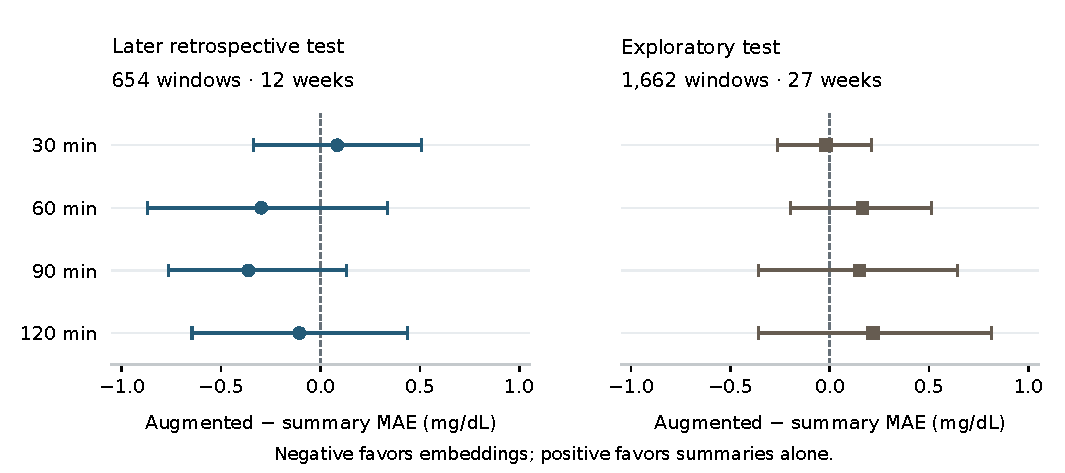
\includegraphics[width=1\linewidth,height=\textheight,keepaspectratio,alt={Paired augmented-minus-summary MAE at all four horizons. Points are measured differences; lines are 95\% percentile intervals from 2,000 paired week-bootstrap draws. Both panels use the same scale. All eight intervals include zero; the later 60-minute comparison is primary.}]{figures/opencgm-comparison.pdf}
\caption{Paired augmented-minus-summary MAE at all four horizons. Points
are measured differences; lines are 95\% percentile intervals from 2,000
paired week-bootstrap draws. Both panels use the same scale. All eight
intervals include zero; the later 60-minute comparison is primary.}
\end{figure}

\subsection{4.2. Exploratory test and tuning
outcomes}\label{exploratory-test-and-tuning-outcomes}

The exploratory slice contains 1,662 windows in 27 weeks. Augmented
Ridge increased MAE at 60, 90 and 120 minutes by 0.17, 0.15 and 0.22
mg/dL, respectively. At 30 minutes it reduced MAE by 0.02 mg/dL. All
four intervals include zero. These losses receive the same reporting and
uncertainty calculation as the later-slice improvements.

Validation selected the smallest allowed alpha, 0.001, for summary Ridge
at all horizons. Augmented Ridge selected 31.6228 at 30 minutes and 100
at the other horizons. The predefined grid was not expanded after
examining results. Consequently, the comparison describes performance
under this tuning budget, not an exhaustive search over downstream
models.

\subsection{4.3. Verification of the measurement
chain}\label{verification-of-the-measurement-chain}

Seven synthetic contract tests passed: parity with upstream binning and
exclusion of future input; half-open target boundaries; clock-day
support exclusion and conflict preservation; temporal support purging;
training-only scaling/fitting with test-target perturbation; paired
event-weighted bootstrap agreement; and private-output path enforcement.

A separate saved-artifact verifier checked every retained window against
clock exclusions. It reproduced 64 stratified private histories using
the pinned upstream grid implementation and independently matched 256
horizon targets to observed-bin means. Saved prediction identities,
targets and persistence values matched the input windows. All reported
MAEs, paired differences and intervals matched an explicit-row
implementation of week resampling. These are implementation and
arithmetic checks; they do not validate the checkpoint's claimed
pretraining history or resolve observational limitations.

\section{5. Interpretation and
limitations}\label{interpretation-and-limitations}

\textbf{Incremental utility, not absence of information.} The experiment
found no clear added forecasting value from this frozen representation
under the chosen Ridge readout. It does not show that the embedding
contains no useful information. A linear predictor over a mean-pooled
daily representation tests a particular route from representation to
forecast. The augmented arm also has more input dimensions, so the
result reflects the representation and its fitted readout together.

\textbf{A conditional negative result, not equivalence.} Small point
estimates and intervals spanning zero do not prove equal performance.
Only 12 weeks contribute to the later test. The reported uncertainty
omits training variation, alternative split choices and possible
dependence across weeks. No clinically meaningful equivalence margin was
specified.

\textbf{Selection and availability.} Complete future target observation
is known only retrospectively, and history eligibility favors
well-recorded periods. The resulting errors do not estimate continuous
deployment performance over missing or ambiguous intervals. Export
timestamps also do not establish when each reading would have reached a
live prediction system. The last-bin convention gives all arms the same
available input here, but it is not a claim about optimal real-time
timing.

\textbf{One person and a changing treatment context.} Thousands of
windows from one person do not constitute thousands of independent
participants. The glucose trajectory was recorded under the author's
ongoing treatment and behavior. This study neither randomizes that
context nor evaluates model-guided treatment changes. It cannot identify
causes of glucose changes, infer insulin sensitivity from prediction
accuracy, or establish transfer to other people.

\textbf{One community artifact and a different task.} The released
weights are a single checkpoint with maintainer-reported provenance.
Hash matching establishes which bytes were evaluated. It does not make
the artifact an official GlucoFM release, independently verify its
training corpus, or turn this fixed-time forecasting task into a
reproduction of the original phenotype or meal-response evaluations
{[}1, 2{]}.

\section{6. Conclusion}\label{conclusion}

On the author's eligible later glucose windows, eight glucose/time
summaries supported a stronger predictor than persistence, while adding
the pinned OpenCGM-StateEvent embedding produced only small,
inconsistent changes. The primary 60-minute difference was \ensuremath{-}0.30 mg/dL,
with a paired interval spanning zero. The defensible conclusion is
specific: \textbf{this frozen community checkpoint did not establish
added predictive value beyond these summaries under this evaluation}.
The broader question of physiological understanding remains unanswered
by forecast accuracy alone.

\section{Data, code and assistance}\label{data-code-and-assistance}

The author is the sole participant and data source. Raw CareLink
exports, window-level features, embeddings and predictions remain
private. All inference was local. The accompanying project files contain
the analysis code, pinned source and artifact references, synthetic
tests, and non-reconstructive aggregate outputs. Complete numerical
replication requires the private inputs; the manuscript and its figure
can be rebuilt from aggregates alone. A permanent public code-archive
identifier has not been assigned at this checkpoint.

Code, analysis checks and manuscript preparation used AI assistance.
Numerical claims were checked against executable outputs and cited
source records; agreement between assistants was not treated as
validation. The earlier baseline article and its corrections remain in
the project history.

\section{References}\label{references}

\begin{enumerate}
\def\labelenumi{\arabic{enumi}.}
\tightlist
\item
  Zechen Li et al.~\emph{GlucoFM: A Dual-Stream Foundation Model for
  Continuous Glucose Monitoring.} arXiv:2605.30865, version 2, 25 August
  2026. \url{https://arxiv.org/abs/2605.30865v2}.
\item
  Stephane Fourdrinier. \emph{OpenCGM-StateEvent: model card and
  released encoder.} 2026. Hugging Face repository
  {\ttfamily\nolinkurl{sfourdrinier/opencgm-stateevent}}, revision
  {\ttfamily\nolinkurl{6c53e572c2dafcb0b030f2e1aa4f3a2a8d7f7ca3}}.
  \href{https://huggingface.co/sfourdrinier/opencgm-stateevent/blob/6c53e572c2dafcb0b030f2e1aa4f3a2a8d7f7ca3/README.md}{Pinned
  model card}.
\item
  Stephane Fourdrinier. \emph{OpenCGM: source and ONNX export
  implementation.} 2026. GitHub repository
  \texttt{sfourdrinier/opencgm}, revision
  {\ttfamily\nolinkurl{bcf8ac2dfca00f8fb3c7728fb2a3a2bd2803bebf}}.
  \href{https://github.com/sfourdrinier/opencgm/tree/bcf8ac2dfca00f8fb3c7728fb2a3a2bd2803bebf}{Pinned
  source}.
\end{enumerate}

\section{Appendix A. Exact encoder and protocol
identity}\label{appendix-a.-exact-encoder-and-protocol-identity}

\textbf{Encoder SHA-256:}

{\ttfamily\nolinkurl{b1349deffd15ab62a5a98d7c7c4a7e143bcf1dee7ad745b1e05533ff54f34768}}

\textbf{Frozen protocol-section SHA-256:}

{\ttfamily\nolinkurl{3cc2fd06755d644bdc1a44efdb83d17c62922472b4a06ad8183569a2f69853bb}}

The encoder file is 1,991,782 bytes, opset 17. Its inputs are
\texttt{values} and \texttt{mask}, float32 arrays \texttt{{[}B,288{]}},
and \texttt{circadian\_start}, int64 \texttt{{[}B{]}}. The start index
is the integer part of local minutes since midnight divided by five. The
output is \texttt{embedding}, float32 \texttt{{[}B,128{]}}. Missing
values are finite zeros with mask zero; NaN fill is not part of the
tested contract.

For observed mask \(m_j\), values \(x_j\) and \(n=\sum_jm_j\), the
source's internal normalization uses

\[
\mu=\frac{\sum_jm_jx_j}{n+\epsilon},\quad
v=\frac{\sum_jm_j(x_j-\mu)^2}{n+\epsilon},\quad
\tilde x_j=\frac{m_j(x_j-\mu)}{\max(\sqrt{v+\epsilon},10^{-4})},
\qquad \epsilon=10^{-6}.
\]

An all-unobserved window returns zeros at this normalization step. The
full encoder may still emit a nonzero embedding. The source paths
establishing the contract are \texttt{data/grid.py},
\texttt{data/timestamps.py}, {\ttfamily\nolinkurl{model/causal_gaussian.py}},
\texttt{model/reference.py} and \texttt{model/encoder.py} under
{\ttfamily\nolinkurl{src/opencgm_stateevent/}}, plus
{\ttfamily\nolinkurl{scripts/export_encoder_onnx.py}}. Their individual hashes and
the complete artifact metadata are recorded in
{\ttfamily\nolinkurl{assets/article/opencgm-provenance.json}}.

The model card labels the encoder CC-BY-NC-4.0 and the source
Apache-2.0. It reports pretraining on Stanford, Shanghai T2DM, Big Ideas
and Colas, while recording unresolved source licensing for Stanford
{[}2, 3{]}. The separate bundled probe heads are not used in this study.

\section{Appendix B. Reproduction and evidence
map}\label{appendix-b.-reproduction-and-evidence-map}

Commands below run from the project root using the recorded Python
3.14.3 environment. Runtime dependencies are pinned in
{\ttfamily\nolinkurl{carelink-local/requirements-opencgm.txt}}: NumPy 2.5.3, pandas
3.0.6, ONNX 1.23.0 and ONNX Runtime 1.30.0. The measured runtime is
macOS arm64 with the CPU execution provider.

\begin{verbatim}
PY=carelink-local/.venv/bin/python
$PY carelink-local/archive_inventory.py private-data/carelink/*.csv \
  --output assets/article/archive-inventory.json
$PY carelink-local/clock_audit.py
$PY carelink-local/prepare_opencgm.py
$PY carelink-local/opencgm_comparison.py smoke
$PY -m unittest discover -s carelink-local \
  -p 'test_opencgm_comparison.py' -v
$PY carelink-local/opencgm_comparison.py build
$PY carelink-local/opencgm_comparison.py score
$PY carelink-local/verify_opencgm_run.py
\end{verbatim}

The inventory command reproduces the archive audit; the comparison
commands correspond to the executed stages. The frozen protocol remains
in \texttt{TANDEM.md}. Aggregates under \texttt{assets/article/} provide
the evidence chain: {\ttfamily\nolinkurl{archive-inventory.json}} for source coverage
and midnight aggregates; \texttt{clock-audit.json} for collisions and
exclusions; {\ttfamily\nolinkurl{opencgm-provenance.json}} for identity;
\texttt{opencgm-smoke.json} for synthetic inference;
\texttt{opencgm-build.json} for eligibility and splits;
\texttt{opencgm-results.json} for every arm, horizon, interval and
chosen alpha; and \texttt{opencgm-checks.json} for independent
saved-artifact verification.

The results JSON also contains absolute-MAE intervals and paired
comparisons against persistence for both periods. All published tables
and the figure are checked against that aggregate. Generating the
preprint does not rerun model selection, alter the frozen protocol, or
read private windows.
\end{document}
